 \documentclass[25pt, a0paper, portrait, margin=0mm, innermargin=10mm,
     blockverticalspace=7mm, colspace=8mm, subcolspace=8mm]{tikzposter} %Default values for poster format options.

 \tikzposterlatexaffectionproofoff % not show small comment on how the poster
 %was made at bottom of poster

\usepackage{url}
\usepackage{algorithmic}
\usepackage{algorithm}

\renewcommand{\algorithmicrequire}{\textbf{In:}}
\renewcommand{\algorithmicensure}{\textbf{Out:}}

\usepackage{amsmath}
\usepackage{amssymb}
\usepackage{enumitem}
% make the itemize compact
\setlist[itemize]{nosep}
\setlist[enumerate]{itemsep=2mm}
%\usepackage{caption}
\usepackage[mathscr]{eucal}
\usepackage{graphicx}

%%%%%%%%%%%%%%%%%%%%%%%%%%%%%% User specified LaTeX commands.

\usepackage{amsfonts}
\usepackage{amsthm}
\usepackage{amssymb}
\usepackage{lmodern}
\usepackage{pifont}
\usepackage{setspace}
\usepackage{tikz}
%\usetikzlibrary{bayesnet}
\usetikzlibrary{shapes.geometric,decorations.markings}
\usepackage{xcolor}

%\usepackage{epstopdf}
%\usepackage{auto-pst-pdf}
%\usepackage{subfig}

%\everymath{\color{mathcolor}}
%\everydisplay{\color{mathcolor}} 


\newcommand{\diag}{\mathop{\mathrm{diag}}}
\newcommand{\trace}{\mathop{\mathrm{tr}}}
\newcommand{\median}{\mathop{\mathrm{median}}}
%\newcommand{\proj}{\mathop{\mathrm{proj}}}


\newcommand{\bx}{\mathbf{x}}				% all variables
%\newcommand{\factor}{\psi}				% factor
\newcommand{\factor}{f}				% AG: made this f for consistency
\newcommand{\outV}{V}                         %AG: output variable of a factor
\newcommand{\fis}[1]{\mathrm{ne}(#1)}   	% index set for variables connected to  factor
\newcommand{\fx}[1]{ \mathbf{x}_{\mathrm{ne}(#1)} }   	% variables of a factor
\newcommand{\xin}{\mathbf{x}_{ \mathrm{in} }} 			% parents of directed factor
\newcommand{\xout}{\mathbf{x}_{ \mathrm{out} }}			% child of directed factor
\newcommand{\msg}[2]{m_{#1 \rightarrow #2}}			% message from arg1 to arg2
\newcommand{\approxMsg}[3]{M_{#1 \rightarrow #2}^{#3}}			% message from arg1 to arg2
\newcommand{\uncert}{{\mathfrak v}}          %%AG: variable used to denote uncertainty
\newcommand{\uncertaintyMsg}[3]{{\mathfrak V}_{#1 \rightarrow #2}^{#3}}			% message from arg1 to arg2
\newcommand{\diffd}{\mathrm{d}}
%\newcommand{\proj}{\mathrm{proj}}   %AG: replaced with notation using less space

%\newcommand{\proj}{\mathbb{Q}}


\newcommand{\projP}[1]{\mathrm{proj} \left [ #1 \right]}   
\DeclareMathOperator*{\proj}{\text{proj}} % WJ defined this

\newcommand{\argmin}[1]{\mathrm{arg}\mathrm{min}_{#1}}
%\newcommand{\kld}[2]{\mathrm{KL} \left [ #1 || #2 \right ]}
%\newcommand{\expectationE}[2]{ \mathbb{E}_{#2}  \left[ #1 \right] }

% random features stuff
\newcommand{\feax}{\mathsf{x}}
\newcommand{\feaX}{\mathsf{X}}
\newcommand{\feay}{\mathsf{y}}
\newcommand{\feaY}{\mathsf{Y}}

\newcommand{\figref}[1]{Fig.~\ref{#1}}
\newcommand{\secref}[1]{Section~\ref{#1}}
\newcommand{\tabref}[1]{Table.~\ref{#1}}

% Gatsby Unit, University College London$^1$ \\
% \vspace*{2mm}
% University of Oxford$^2$ \\
% \texttt{ \{wittawatj,  arthur.gretton\}@gmail.com}, \, \texttt{nheess@nhuk.de} \\ 
% \texttt{ali@arkitus.com}, \, \texttt{balaji@gatsby.ucl.ac.uk},\\
% \texttt{dino.sejdinovic@gmail.com},\, \texttt{z.szabo@ucl.ac.uk}


\graphicspath{{../img/}}
%%%%%%%%%%%%%%
\title{Kernel-Based Just-In-Time Learning For Passing Expectation Propagation Messages  }
%\title{Kernel-Based Just-In-Time Learning For Expectation Propagation }
    \author{\hspace{65mm} Wittawat Jitkrittum,$^1$ \, Arthur Gretton,$^1$ \, Nicolas Heess, \, S. M. Ali Eslami \, \newline
Balaji Lakshminarayanan,$^1$ \, Dino Sejdinovic$^2$ and \, Zolt{\'a}n Szab{\'o}$^1$  
}
\institute{%
Gatsby Unit, University College London$^1$ 
\hspace{3cm}
University of Oxford$^2$
%\newline Google DeepMind$^2$
}

% -- PREDEFINED THEMES ---------------------- %
% Choose LAYOUT:  Default, Basic, Rays, Simple, Envelope, Wave, Board, Autumn, Desert,
\usetheme{Board}
%\usenotestyle{Corner}
\usenotestyle{Sticky}
\colorlet{notebgcolor}{yellow!30!white}
\colorlet{notefrcolor}{notebgcolor}
%\usetheme{Autumn}
%\usetitlestyle{Default}
%\useblockstyle{Minimal}
%\colorlet{titlefgcolor}{green}
%\usecolorstyle[colorPalette=BrownBlueOrange]{Germany}
%\usecolorstyle[colorPalette=BlueGrayOrange]{Spain}
%\usecolorstyle{Australia}
%\usecolorstyle{Britain}
%\usecolorstyle{Sweden}
%\usecolorstyle{Russia}

\definetitlestyle{MyTitleStyle}{
   width=0.97\paperwidth, roundedcorners=0, linewidth=0pt, innersep=8mm,
   titletotopverticalspace=5mm, titletoblockverticalspace=10mm,
   titlegraphictotitledistance=0pt, titletextscale=1
}{}
\usetitlestyle{MyTitleStyle}

\settitle{ \centering \vbox{
\@titlegraphic \\[\TP@titlegraphictotitledistance] \centering
\color{titlefgcolor} \vspace{1em} {\fontsize{54}{42} \textbf{\@title} \par}
%\color{titlefgcolor} {\huge \textbf{\@title} \par}
\vspace*{1em}
{\huge \@author \par} \vspace*{1em} {\LARGE \@institute}
}}


\colorlet{mathcolor}{blue!70!black}
% \newcommand{\Smile}{\Simley{0.6}{green!20}}
% \newcommand{\Frown}{\Simley{-0.53}{red!15}}
\newcommand{\cmark}{\ding{51}}%
\newcommand{\xmark}{\ding{55}}%
\newcommand{\Smile}{ {\large \textcolor{green}{\cmark}} }
\newcommand{\Frown}{ {\large \textcolor{red}{\xmark}} }

\newcommand{\Vskip}{\vspace{5mm}}
%\newenvironment{wideitemize}{\itemize\addtolength{\itemsep}{100pt}}{\enditemize}

% make body text's font bigger.
% compile font_gen.tex first.
% http://tex.stackexchange.com/questions/243678/how-to-make-tikzposter-work-with-font-sizes-larger-than-25pt
\makeatletter
%\input{theguy36pt.clo}
\input{theguy27pt.clo}
\makeatother 
%%%%%%%%%%%%%%%%%%%%%%%%%%%%%%%%%%%%%%
\begin{document}
\maketitle[width=0.95\paperwidth ]
\begin{columns}
%==================================
\column{0.5}
%==================================
%--------------------------
\block[roundedcorners=40]{Introduction}{
%--------------------------
EP is a widely used message passing based inference algorithm. 
\begin{itemize}
    \item \textbf{Problem}: Expensive to compute outgoing from incoming messages.
    \item \textbf{Goal}: Speed up computation by a cheap regression function
        (message operator): 
    \begin{equation*}
        \text{incoming messages} \mapsto \text{outgoing message}.
    \end{equation*}
\end{itemize}
%
\vspace*{-8mm}
\textbf{Merits}:
\begin{itemize}
    \item Efficient online update of the operator during inference.
    \item Uncertainty monitored to invoke new training examples when needed. 
    \item Automatic random feature representation of incoming messages.
\end{itemize}
}

%--------------------------
\block{Expectation Propagation (EP)}{
%--------------------------
%\definecolor{mygreen}{RGB}{0,100,0}
\colorlet{mygreen}{green!52!black}

Under an approximation that each factor fully factorizes, an outgoing EP
message $\textcolor{mygreen}{m_{f\rightarrow V_i}}$ takes the form
\vspace{5mm}
%% \begin{align*}
%% \frac{\proj\left[\int d\mathcal{V}\backslash\{v\}\, f(\mathcal{V})\prod_{V'\in\mathcal{V}}m_{V'\rightarrow f}(v')\right]}{m_{V\rightarrow f}(v)}:=\frac{q_{f\rightarrow V}(v)}{m_{V\rightarrow f}(v)}
%% \end{align*}
 
\tikzstyle{every picture}+=[remember picture]
\tikzstyle{na} = [baseline=-.5ex]

%\tikz[na] \node[fill=blue!10,draw,circle] (n1) {}; 
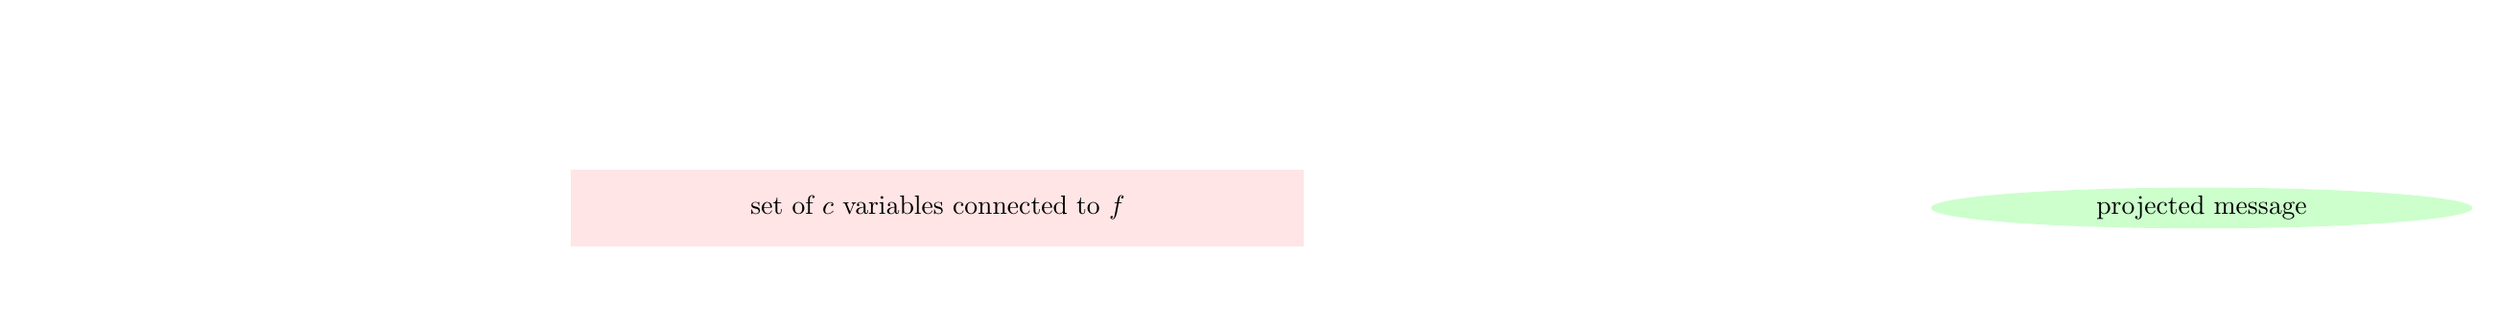
\begin{tikzpicture}[scale=1.2]
\draw[help lines, white, opacity=0] (0, -1) grid (25, 2); 
%\draw[very thick, <->] (1,0) to (0,0) to (0,1); 
\node (v_def) [right, fill=red!10, inner sep=10pt, align=center, text
width=9cm] at (6, 0) {set of $c$ variables connected to $f$};
\node (proj_msg_def) [right, fill=green!20, ellipse, inner sep=1pt,
align=center, text width=5cm] at (21, 0) {projected message};
\end{tikzpicture}

\begin{align*}
    \textcolor{mygreen}{m_{f\rightarrow V_i}(v_i)} = 
  \frac{
	  \tikz[baseline]{
	  \node[fill=blue!7,anchor=base] (proj){ $\proj$ };
  }
  \left[\int d\mathcal{V}\backslash\{v_i\}\, f(
	  \tikz[baseline]{
		  \node[fill=red!10,anchor=base, inner sep=3pt] (v_set){$\mathcal{V}$};
	  }
  )\prod_{j=1}^c 
    %\color{red}
	  \tikz[baseline]{
		  \node[fill=orange!10!white, anchor=base] (inc) 
          {\textcolor{red}{$m_{V_j \rightarrow f}(v_j)$}} ; % end numerator
	  }
    %\color{mathcolor}
  \right]}{m_{V_i\rightarrow f}(v_i)} := 
  \frac{	
  \tikz[baseline]{
	  \node[fill=green!20,anchor=base] (projected)
	  { $q_{f\rightarrow V_i}(v_i)$ };
  }
  }{m_{V_i \rightarrow f}(v_i)}  
\end{align*}

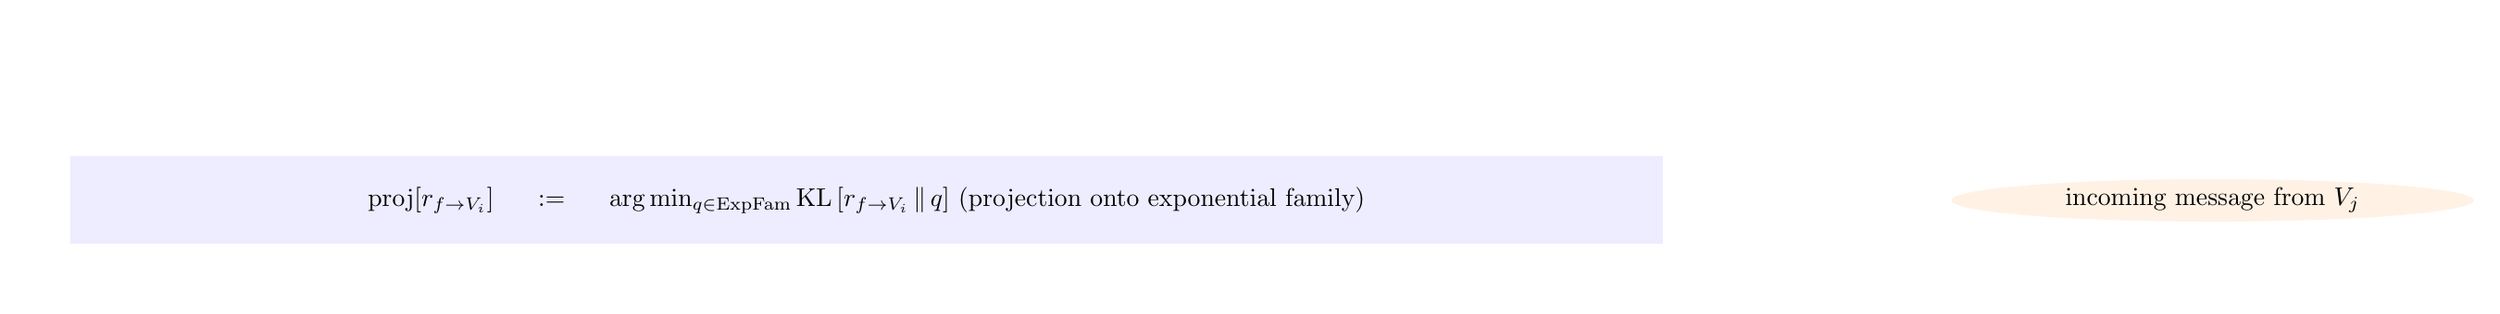
\begin{tikzpicture}[scale=1.2]
\draw[help lines, white, opacity=0] (0, -1) grid (25, 2);
%\draw[very thick, <->] (1,0) to (0,0) to (0,1); 
\node (projdef) [right, fill=blue!7, rectangle, inner sep=12pt, align=center,
text width=21cm]  at (0.5, 0) {$\proj[r_{f \rightarrow
V_i}]:=\arg\min_{q\in\text{ExpFam}}\text{KL}\left[r_{f \rightarrow V_i}\,\|\,
q\right]$ (projection onto exponential family)}; 
%
\node (incdef) [right, fill=orange!10, ellipse, inner sep=1pt, align=center, text
width=5cm]  at (22, 0) {incoming message from $V_j$}; 
\end{tikzpicture}


% Now it's time to draw some edges between the global nodes. Note that we
% have to apply the 'overlay' style.
\begin{tikzpicture}[overlay]
   \draw[->, line width=3pt] (v_def) edge [bend left] (v_set.north);
   %\draw[->, line width=3pt] (projdef.north) to [out=120, in=-90] (proj.south);
   \draw[->, line width=3pt] (projdef) to [bend left] (proj.south);
   \path[->, line width=3pt] (incdef) edge [bend left] (inc);
   %\path[->, line width=4pt] (proj_msg_def) edge [out=80, in=220] (projected.south west);
   \path[->, line width=3pt] (proj_msg_def) edge [bend left] (projected.north);
\end{tikzpicture}

\begin{tikzfigure}[]
    \vspace{-15mm}
%\centering
 %\subfloat[ Message passing on a factor graph.]{
 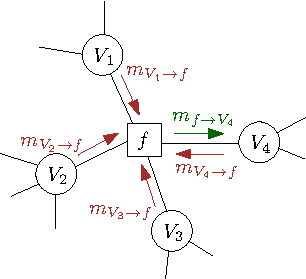
\includegraphics[width=17cm]{img/factor_graph-crop.pdf}
 %}
 \hspace{1cm}
 %
 %\subfloat[ Projection of $r_{f\rightarrow V}$ to a Gaussian]{
 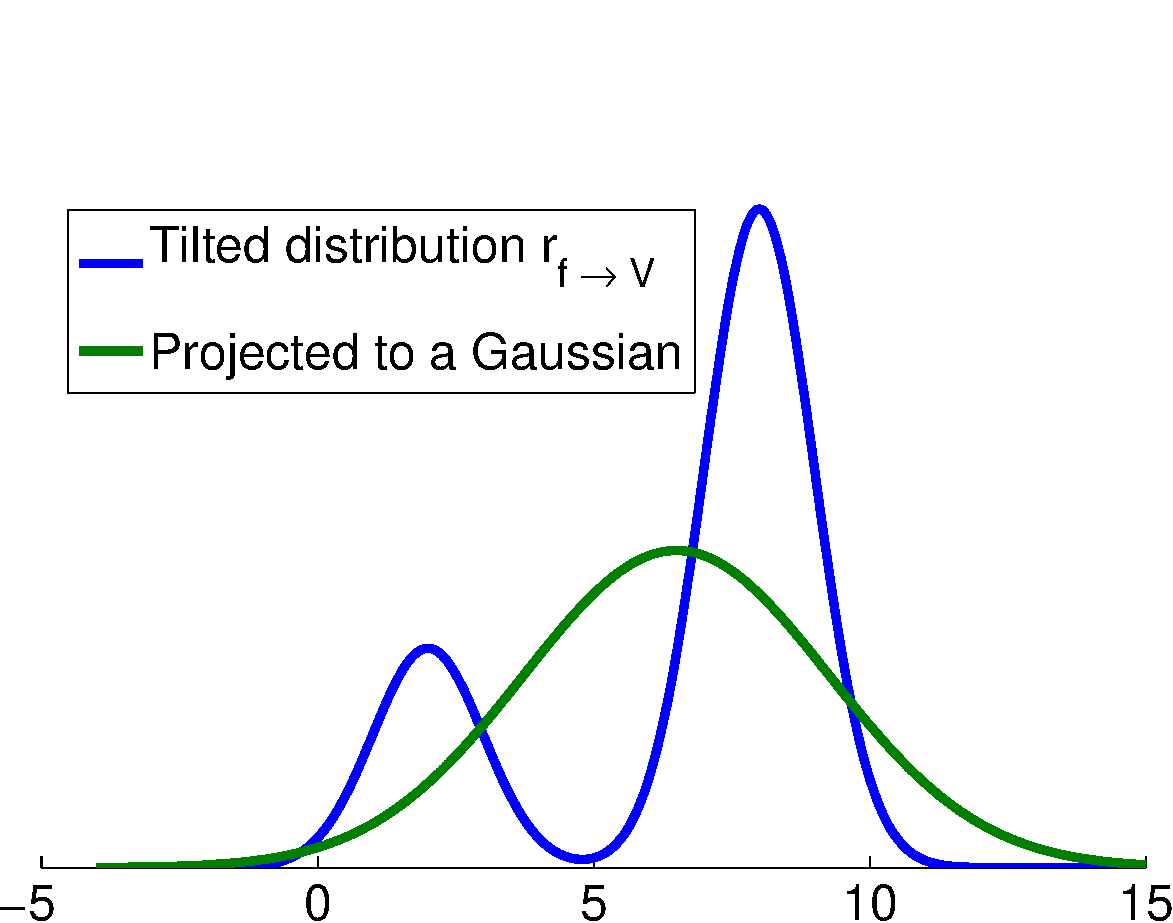
\includegraphics[width=17cm]{img/proj_demo-crop.pdf}
 %}
 %
\end{tikzfigure}
%
\textbf{Projected message:} 

\begin{itemize}
    \item $q_{f\rightarrow V}(v)=\proj\left[r_{f\rightarrow V}(v)\right] \in
        \text{ExpFam}$ with sufficient statistic $u(v)$.

    \item Find $q_{f\rightarrow V}(v)$ by moment matching: $\mathbb{E}_{q_{f\rightarrow
        V}}\left[u(v)\right]=\mathbb{E}_{r_{f\rightarrow V}}\left[u(v)\right] $.
\end{itemize}

%Let $q_{f\rightarrow V}(v)\in\text{ExpFam}$
%with sufficient statistic $u(v)$. 


%\begin{equation*}
%\mathbb{E}_{q_{f\rightarrow V}}\left[T(v)\right]=\mathbb{E}_{r_{f\rightarrow V}}\left[T(v)\right] \text{(moment matching).}
%\end{equation*}
%
} % end block


%--------------------------
\block{Kernel on Incoming Messages}{
%--------------------------

Propose to incrementally learn during inference a kernel-based EP message operator 
(distribution-to-distribution regression) 
%
\begin{equation*}
    \left[ m_{V_j \rightarrow f}  \right]_{j=1}^c \mapsto q_{f \rightarrow V_i},
\end{equation*}
%
for any factor $f$ that can be sampled. 

\begin{itemize}
    \item Product distribution of $c$ incoming messages: 
        $\mathsf{r}:=\times_{l=1}^c r_{l}$, \hspace{5mm}
        $\mathsf{s}:=\times_{l=1}^c s_{l}$.     
    
    \item Mean embedding of $\mathsf{r}$:
        $\mu_{\mathsf{r}}:=\mathbb{E}_{a \sim \mathsf{r}}k(\cdot,a)$.

    \item Gaussian kernel on (product) distributions. Two-staged random feature
        approximation:
        %\begin{align*}
%&= \exp\left(-\frac{1}{2\gamma^{2}}\left\langle
%  \mu_{\mathsf{r}},\mu_{\mathsf{r}}\right\rangle
%  +\frac{1}{\gamma^{2}}\left\langle
%  \mu_{\mathsf{r}},\mu_{\mathsf{s}}\right\rangle
%  -\frac{1}{2\gamma^{2}}\left\langle
%  \mu_{\mathsf{s}},\mu_{\mathsf{s}}\right\rangle \right).
        %\end{align*}

\begin{equation*}
           \kappa(\mathsf{r}, \mathsf{s}) = 
            \exp\left(-\frac{\|\mu_{\mathsf{r}}-
            \mu_{\mathsf{s}}\|_{\mathcal{H}}^{2}}{2\gamma^{2}}\right)
    %\kappa(\mathsf{r}, \mathsf{s}) 
            \stackrel{\textcolor{red}{1^{st}}}{\approx}\exp\left(-\frac{
        \|\hat{\phi}(\mathsf{r})-\hat{\phi}(\mathsf{s})\|_{D_\mathrm{in}}^{2}}{2\gamma^{2}}\right)
        \stackrel{\textcolor{red}{2^{nd}}}{\approx}
        \hat{\psi}(\mathsf{r})^\top \hat{\psi}(\mathsf{s}).
    \end{equation*}

\end{itemize}
%
} % end block

%--------------------------
\block{Message Operator: Bayesian Linear Regression }{
%--------------------------

\begin{itemize}
    \item \textbf{Input:} $\mathsf{X}=\left(\mathsf{x}_{1}|\cdots|\mathsf{x}_{N}\right)$: 
        $N$ training incoming messages represented as random feature vectors.
    \item \textbf{Output:} $\mathsf{Y}=\left(\mathbb{E}_{r_{\factor\rightarrow
        \outV}^{1}}u(v)|\cdots|\mathbb{E}_{r_{f\rightarrow
        \outV}^{N}}u(v)\right)\in\mathbb{R}^{D_{y}\times N}$: 
        sufficient statistics of outgoing messages.
    \item Inexpensive online updates of posterior mean and covariance.
    \item Bayesian regression gives prediction and predictive variance.
    \item If predictive variance $>$ threshold, query the importance sampling oracle.
\end{itemize}
%\textcolor{red}{code available}

}% end block


 \note[targetoffsetx=-6.0cm, targetoffsety=-7cm,rotate=0,
     angle=270,radius=1cm, width=28cm,innersep=0.9cm]{
         Contact: \url{wittawat@gatsby.ucl.ac.uk}.
         
         Code download: 
         \url{http://github.com/wittawatj/kernel-ep}.
}
%==================================
\column{0.5}
%==================================

%--------------------------
\block{Two-Staged Random Features }{
%--------------------------
% \begin{algorithm}[t]
% \caption{Construction of two-stage random features for $\kappa$}
% \label{algo:random_features_kgg}
    \begin{spacing}{1.3}
\begin{algorithmic}[1]
\REQUIRE 
%Joint $\mathsf{r}$ of incoming messages, 
$\mathscr{F}(k)$: Fourier transform of $k$, $D_\mathrm{in}$: \#inner features, 
$D_\mathrm{out}$: \#outer features, $k_\text{gauss}$: Gaussian kernel on
$\mathbb{R}^{D_\mathrm{in}}$
%, outer Gaussian width $\gamma^2$.
\ENSURE Random features $\hat{\psi}(\mathsf{r}) \in \mathbb{R}^{D_\mathrm{out}}$

%\STATE Compute the Fourier transform $\hat{k}$ of the kernel $k$.
\STATE Sample  $\{ \omega_i \}_{i=1}^{D_\mathrm{in}} \overset{i.i.d}{\sim} \mathscr{F}(k)$,
\hspace{2cm}
$\{b_i\}_{i=1}^{D_\mathrm{in}} \overset{i.i.d}{\sim} U[0, 2\pi] $.

%\hspace{10mm} $\{b_i\}_{i=1}^{D_\mathrm{in}} \overset{i.i.d}{\sim} U[0, 2\pi] $.

%\STATE Sample $\{b_i\}_{i=1}^{D_\mathrm{in}} \overset{i.i.d}{\sim} U[0, 2\pi] $.

\STATE $\hat{\phi}(\mathsf{r}) = \sqrt{\frac{2}{D_\mathrm{in}}} \left(
\mathbb{E}_{\mathsf{x \sim \mathsf{r}}} 
\cos(\omega_{i}^{\top}x+b_{i} ) \right)_{i=1}^{D_\mathrm{in}} \in \mathbb{R}^{D_\mathrm{in}}$ \\
%\STATE  $\hat{\phi}(p)=\mathbb{E}_{p(x)}\sqrt{\frac{2}{D_\mathrm{in}}}\left(\cos\left(\omega_{1}^{\top}x+b_{1}\right),\ldots,\cos\left(\omega_{D_\mathrm{in}}^{\top}x+b_{D_\mathrm{in}}\right)\right)^{\top}$.
%If $\mathsf{r}(x)=\mathcal{N}(x;m, \Sigma )$,  \\
%$\hat{\phi}( \mathsf{r}) =  \sqrt{\frac{2}{D_\mathrm{in}}} \left( \cos(\omega_{i}^{\top}m +b_{i}) \exp 
%\left(-\frac{1}{2}\omega_{i}^{\top}\Sigma \omega_{i} \right) \right)_{i=1}^{D_\mathrm{in}}$.
% \small
% \begin{equation*}
% \hat{\phi}( \mathsf{r}) = \sqrt{\frac{2}{D_\mathrm{in}}} \left( \cos(\omega_{i}^{\top}m +b_{i}) \exp 
% \left(-\frac{1}{2}\omega_{i}^{\top}\Sigma \omega_{i} \right) \right)_{i=1}^{D_\mathrm{in}}.
% \end{equation*}
%
%Even if $p$ is not a normal distribution, we may still use it as an approximation.
%
\STATE Sample $\{ \nu_i \}_{i=1}^{D_\mathrm{out}} \overset{i.i.d}{\sim}
\mathscr{F}({k}_{\text{gauss}}(\gamma^{2}))$, \hspace{2cm}
$\{c_i\}_{i=1}^{D_\mathrm{out}} \overset{i.i.d}{\sim} U[0, 2\pi] $.

%\hspace{10mm} 
%\STATE Sample $\{c_i\}_{i=1}^{D_\mathrm{out}} \overset{i.i.d}{\sim} U[0, 2\pi] $.

%i.e., Fourier transform of a Gaussian kernel with width $\gamma^2$.
\STATE $\hat{\psi}(\mathsf{r}) = \sqrt{\frac{2}{D_\mathrm{out}}} \left(  
\cos(\nu_{i}^{\top} \hat{\phi}(\mathsf{r}) + c_{i} ) \right)_{i=1}^{D_\mathrm{out}} \in 
\mathbb{R}^{D_\mathrm{out}}$
\end{algorithmic}
\end{spacing}
% \end{algorithm}

} % end block

%--------------------------
\block{ Experiment 1: Uncertainty Estimates}{
%--------------------------
    \vspace{-8mm}
\begin{center}
%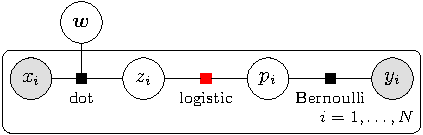
\includegraphics[width=20cm]{binary_logistic_regression-crop}
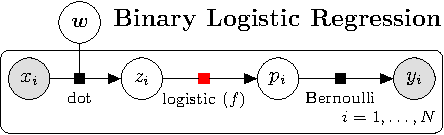
\includegraphics[width=21cm]{img/binlog_graph_title-crop}
\end{center}

\begin{itemize}

\item Approximate the logistic factor: 
    $f(p|z) = \delta\left(p-\frac{1}{1+\exp(-z)}\right)$. 
    %\begin{align*}
    %\msg{z_i}{\factor} &= \mathcal{N}(z_i; \mu, \sigma^2), \hspace{2cm}
    %\msg{p_i}{\factor} = \text{Beta}(p_i; \alpha, \beta). 
    %\end{align*}
    %\vspace{-10mm}
\item Incoming messages: 
    $\msg{z_i}{\factor} = \mathcal{N}(z_i; \mu, \sigma^2), \hspace{2cm}
    \msg{p_i}{\factor} = \text{Beta}(p_i; \alpha, \beta). $
\item Training set = messages collected from 20 EP runs on toy data.

\begin{tikzfigure}
\centering
  %\subfloat[Parameters of $\msg{z_i}{\factor}$ \label{fig:logistic_uncertainty_test}]{
  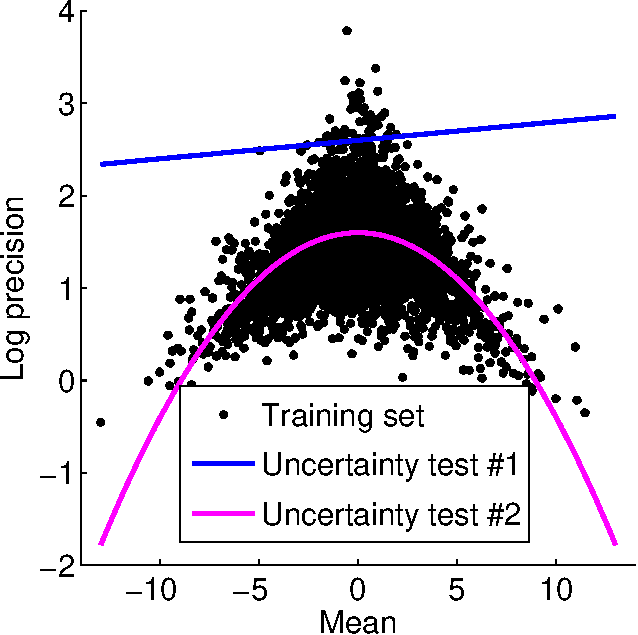
\includegraphics[width=13cm]{uncertainty/logistic_uncertainty_test-crop}
  %}
  \hspace{3cm}
  %
  %\subfloat[Uncertainty estimates \label{fig:logistic_uncertainty_all}]{
      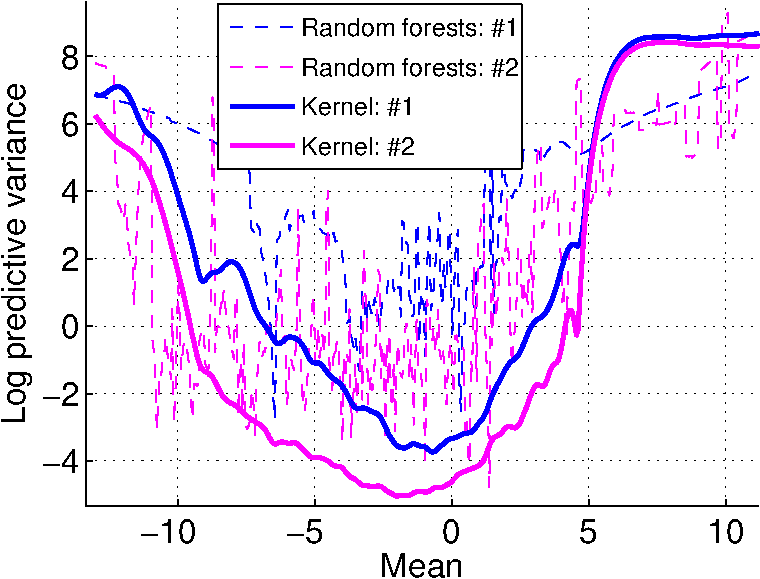
\includegraphics[width=13cm]{uncertainty/logistic_uncertainty_all-crop}
  %\hspace{1.5cm}
  %}
  %
  %\caption{   
  %Eslami et. al.'s random forests (KL-based agreement of predictions of different trees) 
  %on the two uncertainty test sets shown. For testing, we fix the other incoming message 
  %%$\msg{p_i}{\factor}$ to $\text{Beta}(p_i; 1, 2)$.
  %}

  %\label{fig:logistic_uncertainty}
\end{tikzfigure}

\item \#Random features: $D_{in} = 300$ and $D_{out} = 500$.
\end{itemize}

} % end block

%--------------------------
\block{ Experiment 2: Classification Errors}{
%--------------------------

% logistic temporal uncertainty
% \begin{figure}[t]
% \centering
% 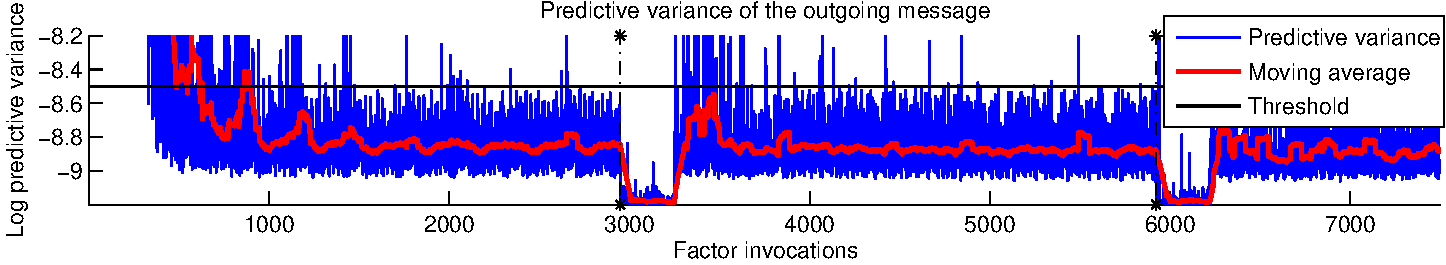
\includegraphics[width=0.95\textwidth]{online/logistic_temporal_uncertainty-crop}
% \caption{Uncertainty estimate of KJIT in its prediction of outgoing messages at each factor invocation,
% for the binary logistic regression problem. The black dashed lines indicate the start 
% of a new inference problem.
% \label{fig:logistic_temporal_uncertainty}
% }
% \end{figure}

    Fix true $\boldsymbol{w}$. Sequentially present 30 problems. Generate
    $\{(x_i, y_i)\}_{i=1}^{300}$ for each.  
        %
\begin{tikzfigure}
    %\vspace{5mm}
  \centering
  %\subfloat[Test error \label{fig:logistic_01_loss}]{
  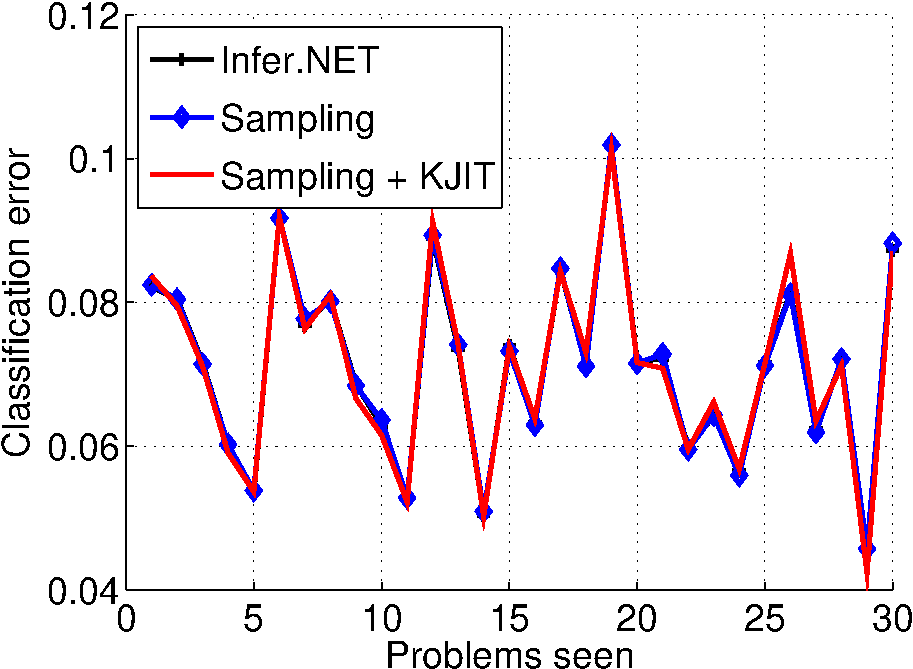
\includegraphics[width=13cm]{online/logistic_01_loss-crop}
  %}
  \hspace{3cm}
  %\subfloat[Inference time\label{fig:logistic_inference_time}]{
  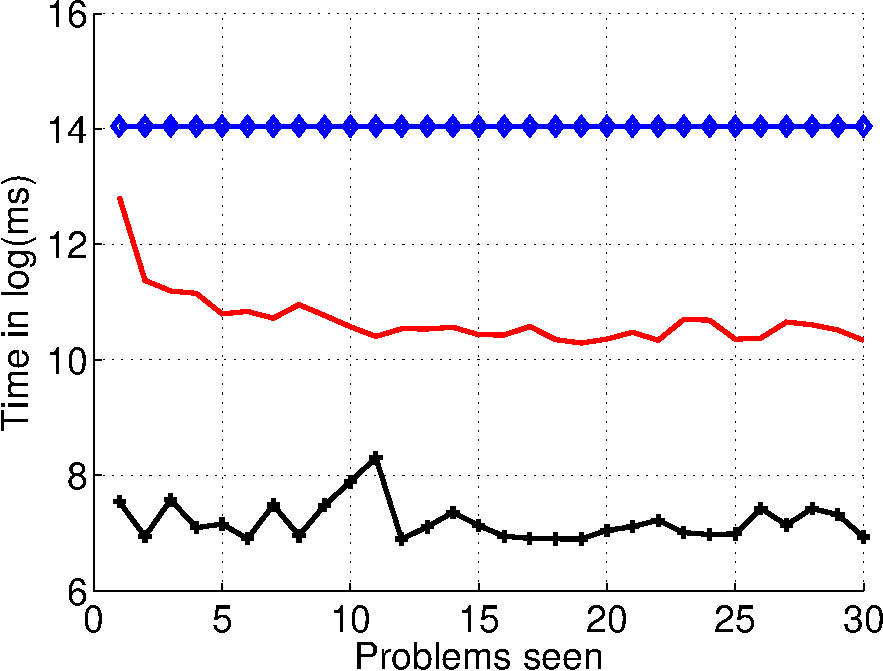
\includegraphics[width=13cm]{online/logistic_inference_time-crop}
  %}
\end{tikzfigure}

\textbf{Sampling + KJIT} = proposed KJIT with an importance sampling oracle.

}% end block

%--------------------------
\block{ Experiment 3: Compound Gamma Factor }{
%--------------------------
Infer posterior of the precision $\tau$ of $x \sim \mathcal{N}(x; 0, \tau^{-1})$ 
from observations $\{x_i\}_{i=1}^N $:
%

\vspace{10mm}

\begin{minipage}{21cm}
      \begin{align*}
         \textcolor{magenta}{r_2} &\sim \mathrm{Gamma}(r_2; s_1, r_1)  \\
         \tau &\sim \mathrm{Gamma}(\tau; s_2, \textcolor{magenta}{r_2} ) \\
         (s_1, r_1, s_2) &= (1, 1, 1).
      \end{align*}
\end{minipage}
%
\begin{minipage}{21cm}
  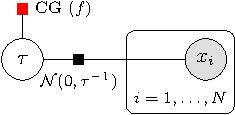
\includegraphics[width=11cm]{img/compound_gamma_graph-crop}
\end{minipage}

\vspace{10mm}

  %
%\begin{subcolumns}
%    \subcolumn{.5}
%      \begin{align*}
%         \textcolor{magenta}{r_2} &\sim \mathrm{Gamma}(r_2; s_1, r_1)  \\
%         \tau &\sim \mathrm{Gamma}(\tau; s_2, \textcolor{magenta}{r_2} ) \\
%         (s_1, r_1, s_2) &= (1, 1, 1).
%      \end{align*}
%  %
%    \subcolumn{.5}
%  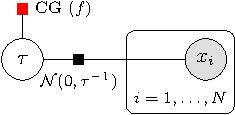
\includegraphics[width=11cm]{img/compound_gamma_graph-crop}
%\end{subcolumns}
%
% compound gamma inferred results and time.
\begin{tikzfigure}
  \centering
% 	\subfloat[Posteriors]{
% 	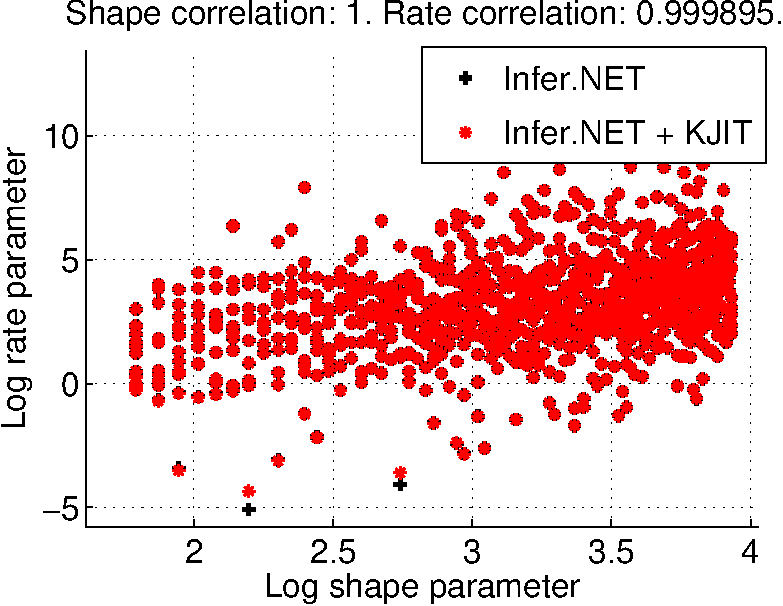
\includegraphics[width=0.49\columnwidth]{img/online/cg_post_corr-crop}
% 	%\missingfigure[figwidth=0.49\columnwidth]{}
% 	}
  %
  %\subfloat[Inferred shape \label{fig:cg_infer_shape}]{
  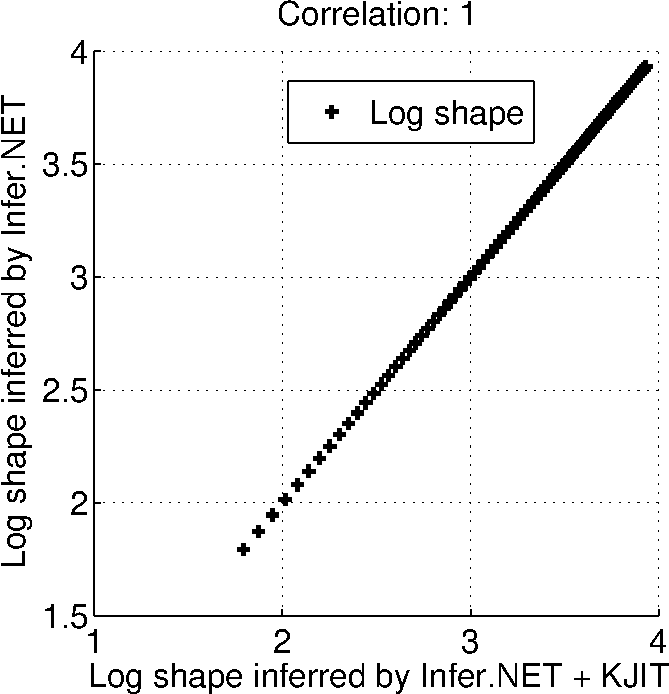
\includegraphics[width=11cm]{online/cg_post_shape-crop}
  %\missingfigure[figwidth=0.49\columnwidth]{}
  %}
  %
  \hspace{1.8cm}
  %\subfloat[Inferred rate \label{fig:cg_infer_rate}]{
  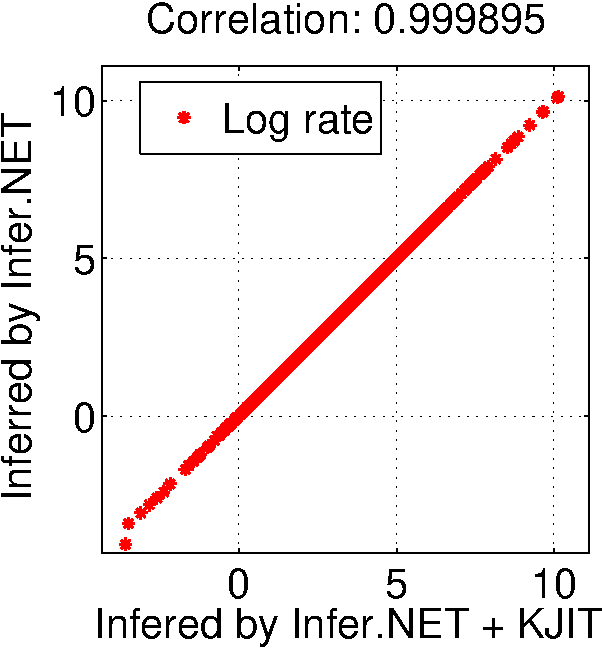
\includegraphics[width=10.5cm]{online/cg_post_rate-crop}
  %\missingfigure[figwidth=0.49\columnwidth]{}
  %}
  %
  \hspace{1.8cm}
  %\subfloat[Inference time\label{fig:cg_infer_time}]{
  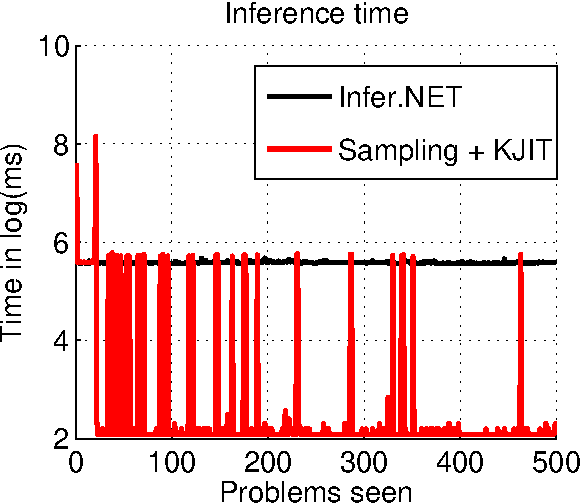
\includegraphics[width=11.2cm]{online/cg_inference_time-crop}
  %}
  %\caption{Shape (a) and rate (b) parameters of the inferred posteriors in 
  %the compound gamma problem. 
  %(c) KJIT is able to infer equally good posterior parameters compared to Infer.NET 
  %while requiring a runtime several orders of magnitude lower. }
\end{tikzfigure}


\begin{itemize}
    \item \textbf{Infer.NET + KJIT} = proposed KJIT with a hand-crafted factor as oracle.
    \item \textbf{Inference quality}: as good as hand-crafted factor; much faster.
\end{itemize}

} % end block


%--------------------------
\block{Acknowledgement}{
%--------------------------
%WJ, AG, BL, and ZSz 
We 
thank the Gatsby Charitable Foundation for the financial
support.
} % end block 

\end{columns}



\end{document}

